\chapter{Aplicações de Transformações Lineares}
As TL têm contribuições significativas para o campo da AL. \cite{strang2010}, renomado matemático e professor do MIT - Massachusetts Institute of Technology, aborda, por exemplo, o processamento de sinais e imagens para compressão, filtragem, reconstrução e análise de dados, a análise de redes e sistemas dinâmicos da engenharia elétrica e ciência da computação, a geometria e a computação gráfica para manipular objetos em espaços tridimensionais, videogames e modelagem em três dimensões, além de cripto segurança e, mais recentemente, análise de dados em decisões gerenciais e aprendizagem de máquina. \nocite{pitombeira1971}

A seguir, baseando em um estudo desenvolvido na Universidade Federal de Alagoas \cite{sirlandro2017}, apresentamos algumas aplicações das TL na área de engenharia.

\section{Posicionamento de Um Braço Robótico}
Para executar atividades repetitivas, perigosas e precisas, um braço robótico, composto por elos e juntas conforme figura 12 é dispositivo dotado de articulações e pode ser programado utilizando aplicações de AL, considerando as variações de posição no plano e no espaço.

\begin{figure}[H]
	\centering
	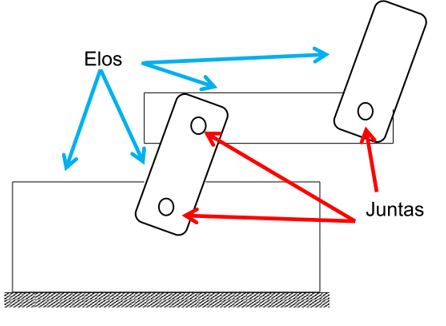
\includegraphics[scale=1.00]{a_robo1.png}
	\caption{Esquema de articulações \cite{sirlandro2017}.}
\end{figure} 

Para representar a aplicação, considere que a figura 13a contém um braço robótico com dois graus de liberdade e seus comprimentos são indicados por $d_1, d_2$ e $d_3$ dos elos, e os ângulos da posição inicial do braço com base no ponto $\mathbf{P}$, nas coordenadas iniciais $(x_0, y_0)$. Na figura 13b, está demonstrada como seria o efeito desse movimento, com o ponto $\mathbf{P}$ na coordenada $(x_1, y_1)$, utilizando as TL.

\begin{figure}[H]
	\centering
	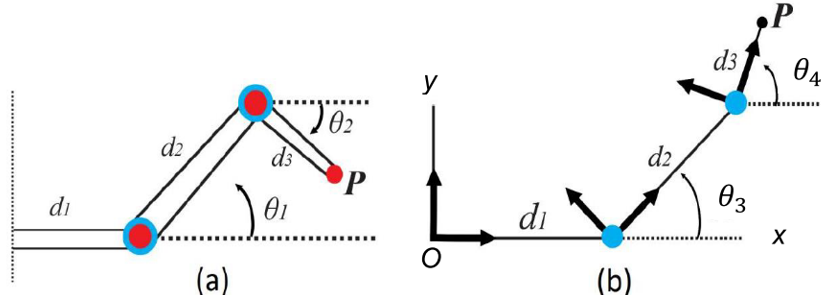
\includegraphics[scale=0.70]{a_robo2.png}
	\caption{Posição inicial e final \cite{sirlandro2017}.}
\end{figure} 

A Figura 14 apresenta o movimento de rotação e translação, e a figura 15 mostra o movimento de translação e rotação, observando que o resultado é diferente de acordo com a ordem aplicada.

\begin{figure}[H]
	\centering
	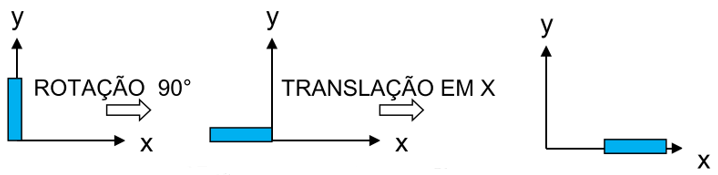
\includegraphics[scale=0.80]{a_robo3.png}
	\caption{Rotação e translação \cite{sirlandro2017}.}
\end{figure} 

\begin{figure}[H]
	\centering
	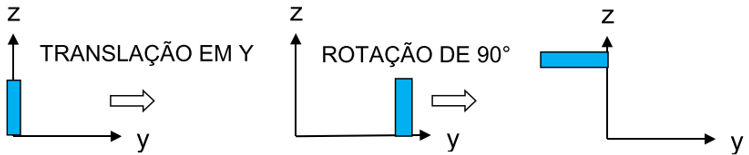
\includegraphics[scale=0.80]{a_robo4.png}
	\caption{Translação e rotação \cite{sirlandro2017}.}
\end{figure} 

Utilizando as TL, consideramos que o sistema adotado como global foi o do antebraço. Denominemos este sistema por $\{\mathbf{A}^0\}$. Onde $\mathbf{e}_1$ e $\mathbf{e}_2$ são os vetores da base canônica do $\mathbb{R}^2$, com origem no ponto $O$ (Figura 13b) e $d_1$ o comprimento do braço e de $\theta_1$ o ângulo que o antebraço faz com o eixo determinado por $\mathbf{e}_1$. Seja $\mathbf{A}_1 = \{f_1, f_2\}$ o sistema local obtido da rotação do sistema $\mathbf{A}_0$ pelo ângulo $\theta_1$ seguida da translação na direção de $\mathbf{e}_1$ por um comprimento $d_1$.

A partir da transformação de rotação, a matriz é representada por

\[
\mathbf{R}_1 = \begin{bmatrix}
	\cos\theta_1 & -\sin\theta_1 & 0\\
	 \sin\theta_1 & \cos\theta_1 & 0\\
	 0 & 0 & 1\\
\end{bmatrix}
\]

\noindent e sua respectiva matriz de translação na direção de $d_1\mathbf{e}_1$ é dada por

\[
\mathbf{T}_1 = \begin{bmatrix}
	1 & 0 & d_1\\
	0 & 1 & 0\\
	0 & 0 & 1\\
\end{bmatrix}
\]

Desta forma, a composição de $\mathbf{T}_1$ com $\mathbf{R}_1$ fica

\[
\mathbf{T}_1\cdot\mathbf{R}_1 = \begin{bmatrix}
	1 & 0 & d_1\\
	0 & 1 & 0\\
	0 & 0 & 1\\
\end{bmatrix}
\begin{bmatrix}
	\cos\theta_1 & -\sin\theta_1 & 0\\
	\sin\theta_1 & \cos\theta_1 & 0\\
	0 & 0 & 1\\
\end{bmatrix}
=
\begin{bmatrix}
	\cos\theta_1 & -\sin\theta_1 & d_1\\
	\sin\theta_1 & \cos\theta_1 & 0\\
	0 & 0 & 1\\
\end{bmatrix}
\]

Considerando que $d_2$ é o comprimento do antebraço e $\theta_2$ o ângulo que não faz com o eixo determinado for $f_1$, o sistema local $\mathbf{A}^2 = \{g_1, g_2\}$ é obtido da rotação do sistema $\mathbf{A}^1$ pelo ângulo $\theta_2$ seguida da translação, na direção de $f_1$, por um comprimento $d_2$, representado pela matriz de rotação

\[
\mathbf{R}_2 = \begin{bmatrix}
	\cos\theta_2 & -\sin\theta_2 & 0\\
	\sin\theta_2 & \cos\theta_2 & 0\\
	0 & 0 & 1\\
\end{bmatrix}
\]

\noindent e pela matriz de translação

\[
\mathbf{T}_2 = \begin{bmatrix}
	1 & 0 & d_2\\
	0 & 1 & 0\\
	0 & 0 & 1\\
\end{bmatrix}
\]

A composição $\mathbf{T}_2\cdot\mathbf{R}_2$ é representada por 

\[
\mathbf{T}_2\cdot\mathbf{R}_2 = \begin{bmatrix}
	1 & 0 & d_2\\
	0 & 1 & 0\\
	0 & 0 & 1\\
\end{bmatrix}
\begin{bmatrix}
	\cos\theta_2 & -\sin\theta_2 & 0\\
	\sin\theta_2 & \cos\theta_2 & 0\\
	0 & 0 & 1\\
\end{bmatrix}
=
\begin{bmatrix}
	\cos\theta_2 & -\sin\theta_2 & d_2\\
	\sin\theta_2 & \cos\theta_2 & 0\\
	0 & 0 & 1\\
\end{bmatrix}
\]

Então houve duas transformações sucessivas partindo do referencial global até o sistema local da mão. Agora partindo uma transformação que leva o referencial $\mathbf{A}^0$ ao referencial $\{\mathbf{A}^2\}$ como mostra a figura 16 abaixo.

\begin{figure}[H]
	\centering
	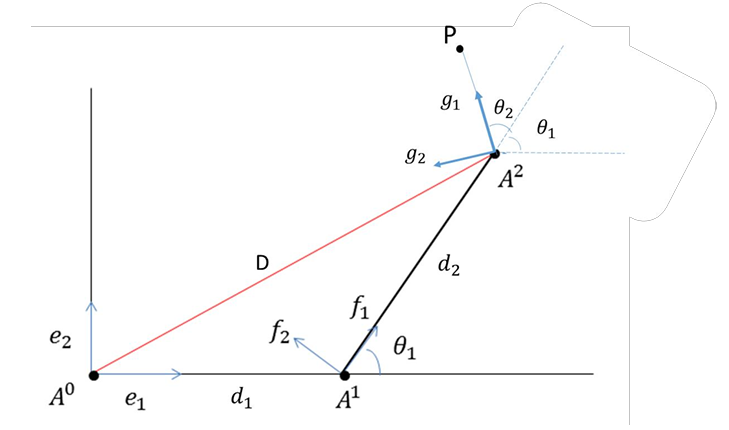
\includegraphics[scale=0.80]{a_robo5.png}
	\caption{Transformação do referencial $\mathbf{A}^0$ para o referencial $\{\mathbf{A}^2\}$ \cite{sirlandro2017}.}
\end{figure} 

Para levar $\mathbf{A}^0$ até $\mathbf{A}^2$ é necessário rotacionar (conforme demonstrado nos capítulos anteriores) e depois transladar, nessa ordem, por uma matriz do tipo

\[
\mathbf{T}\cdot\mathbf{R} = \begin{bmatrix}
	\cos\theta & -\sin\theta & d_1\\
	\sin\theta & \cos\theta & d_2\\
	0 & 0 & 1\\
\end{bmatrix}
\]

Nessa matriz, o ângulo $\theta$ que o referencial $\mathbf{A}^0$ deve ser rotacionado para ficar paralelo ao referencial $\mathbf{A}^2$ é $\theta_1 + \theta_2$. Além disso, note que as coordenadas do vetor translação $t = (t_1, t_2)$ para a transformação $\mathbf{T}\cdot\mathbf{R}$ são

\centerline{$t_1 = d_1 + d_2\cos\theta_1$}

\centerline{$t_2 = d_2\cos\theta_1$}

Então, a matriz de transformação do referencial $\mathbf{A}^0$ para o referencial $\mathbf{A}^2$ pode ser reescrita como 

\[
\mathbf{T}\cdot\mathbf{R} = \begin{bmatrix}
	\cos(\theta_1 + \theta_2) & -\sin(\theta_1 + \theta_2) & d_1 + d_2\cos\theta_1\\
	\sin(\theta_1 + \theta_2) & \cos(\theta_1 + \theta_2) & d_2\sin\theta_1\\
	0 & 0 & 1\\
\end{bmatrix}
\]

\noindent fazendo manipulações algébricas e reduzindo a matriz em um produto temos

\[
\mathbf{T}\cdot\mathbf{R} = \begin{bmatrix}
	\cos\theta_1 & -\sin\theta_1 & d_1\\
	\sin\theta_1 & \cos\theta_1 & 0\\
	0 & 0 & 1\\
\end{bmatrix}
\begin{bmatrix}
	\cos\theta_2 & -\sin\theta_2 & d_2\\
	\sin\theta_2 & \cos\theta_2 & 0\\
	0 & 0 & 1\\
\end{bmatrix}
=
\mathbb{T}_1\cdot\mathbf{R}_1 \bullet \mathbb{T}_2\cdot\mathbf{R}_2
\]

Observe a ordem que este produto deve ser realizado para obtermos a matriz final. Considere agora o referencial local $\mathbf{A}^3$, obtido ao transladarmos o referencial $\mathbf{A}^2$ para o ponto $P$ sem girá-lo. O ponto $P$ está localizado no sistema local $\mathbf{A}^2$ com coordenadas ($d_3, 0)$. É necessário, agora, apenas transladar de $\mathbf{A}^2$ para $P$ por meio da seguinte matriz (o ângulo de rotação é nulo)

\[
\mathbf{T}_3 = \begin{bmatrix}
	1 & 0 & d_3\\
	0 & 1 & 0\\
	0 & 0 & 1\\
\end{bmatrix}
\]

\noindent então, a matriz de transformação geral, M, é dada por 

\[
\mathbf{M} = \begin{bmatrix}
	\cos\theta_1 & -\sin\theta_1 & d_1\\
	\sin\theta_1 & \cos\theta_1 & 0\\
	0 & 0 & 1\\
\end{bmatrix}
\begin{bmatrix}
	\cos\theta_2 & -\sin\theta_2 & d_2\\
	\sin\theta_2 & \cos\theta_2 & 0\\
	0 & 0 & 1\\
\end{bmatrix}
\begin{bmatrix}
	1 & 0 & d_3\\
	0 & 1 & 0\\
	0 & 0 & 1\\
\end{bmatrix}
\]

Para encontrarmos as coordenadas do ponto $P$ no referencial $\mathbf{A}^0$ é necessário aplicar a matriz $\mathbf{M}$ ao vetor $(0, 0, 1)$, origem de $\mathbf{A}^0$. Então o ponto em análise pode ser expresso por

\centerline{$P = \mathbf{M}\cdot(0, 0, 1)$}

\noindent ou seja,

\[
P = \begin{bmatrix}
	\cos\theta_1 & -\sin\theta_1 & d_1\\
	\sin\theta_1 & \cos\theta_1 & 0\\
	0 & 0 & 1\\
\end{bmatrix}
\begin{bmatrix}
	\cos\theta_2 & -\sin\theta_2 & d_2\\
	\sin\theta_2 & \cos\theta_2 & 0\\
	0 & 0 & 1\\
\end{bmatrix}
\begin{bmatrix}
	1 & 0 & d_3\\
	0 & 1 & 0\\
	0 & 0 & 1\\
\end{bmatrix}
\begin{bmatrix}
	0\\
	0\\
	1\\
\end{bmatrix}
\]

\noindent realizando esse produto chegamos a 

\[
P = \begin{bmatrix}
	\cos(\theta_1 + \theta_2) & -\sin(\theta_1 + \theta_2) & d_1 + d_2\cos\theta_1 + cos(\theta_1 + \theta_2)d_3\\
	\sin(\theta_1 + \theta_2) & \cos(\theta_1 + \theta_2) & d_2\sin\theta_1 + \sin(\theta_1 + \theta_2)d_3\\
	0 & 0 & 1\\
\end{bmatrix}
\begin{bmatrix}
	0\\
	0\\
	1\\
\end{bmatrix}
\]

\noindent\textbf{Exemplo 15:} Seja a posição inicial do braço robótico dada pela figura 17, onde $d_1 = 20cm, d_2 = 30cm, d_3 = 14cm, \theta_1 = 60^{\circ}$ e $\theta_2 = -90^{\circ}$.

\noindent\textbf{a)} Determinar as coordenadas do ponto $P$ para esta configuração em relação ao sistema global e \textbf{b)} para $\theta_1 = 45^{\circ}$ e $\theta_2 = 45^{\circ}$.

\begin{figure}[H]
	\centering
	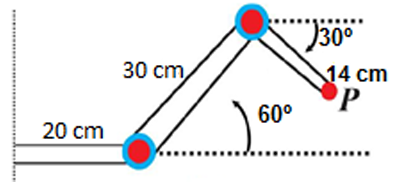
\includegraphics[scale=1.00]{a_robo6.png}
	\caption{Posição inicial do braço robótico $\{\mathbf{A}^2\}$ \cite{sirlandro2017}.}
\end{figure} 

\noindent\textbf{a)} O ponto $P$ é obtido diretamente pela inserção direta dos valores fornecidos

\[
P = \begin{bmatrix}
	\cos(-30) & -\sin(-30) & 20 + 30\cos(60)+ cos(-30)14\\
	\sin(-30) & \cos(-30) & 30\sin(60) + \sin(-30)14\\
	0 & 0 & 1\\
\end{bmatrix}
\begin{bmatrix}
	0\\
	0\\
	1\\
\end{bmatrix}
\]

\[
P = \begin{bmatrix}
	47,12\\
	19\\
	1\\
\end{bmatrix}
\]

\noindent\textbf{b)} O ponto $P$ é obtido diretamente pela inserção direta dos valores fornecidos

\[
P = \begin{bmatrix}
	\cos(90) & -\sin(90) & 20 + 30\cos(45)+ cos(90)14\\
	\sin(90) & \cos(90) & 30\sin(45) + \sin(90)14\\
	0 & 0 & 1\\
\end{bmatrix}
\begin{bmatrix}
	0\\
	0\\
	1\\
\end{bmatrix}
\]

\[
P = \begin{bmatrix}
	41,2\\
	3,2\\
	1\\
\end{bmatrix}
\]

\section{Aplicação das Transformações Lineares na Educação}
É previsto na Base Nacional Comum Curricular \cite{brasil_bncc2018} que estudantes do Ensino Médio adquiram as competências de:

\begin{itemize}
	\item Utilizar estratégias, conceitos e procedimentos matemáticos para interpretar situações em diversos contextos, sejam atividades cotidianas, sejam fatos das Ciências da Natureza e Humanas, das questões socioeconômicas ou tecnológicas, divulgados por diferentes meios, de modo a contribuir para uma formação geral. 
	\item Propor ou participar de ações para investigar desafios do mundo contemporâneo e tomar decisões éticas e socialmente responsáveis, com base na análise de problemas sociais, como os voltados a situações de saúde, sustentabilidade, das implicações da tecnologia no mundo do trabalho, entre outros, mobilizando e articulando conceitos, procedimentos e linguagens próprios da Matemática. 
	\item Utilizar estratégias, conceitos, definições e procedimentos matemáticos para interpretar, construir modelos e resolver problemas em diversos contextos, analisando a plausibilidade dos resultados e a adequação das soluções propostas, de modo a construir argumentação consistente. 
	\item Compreender e utilizar, com flexibilidade e precisão, diferentes registros de representação matemáticos (algébrico, geométrico, estatístico, computacional etc.), na busca de solução e comunicação de resultados de problemas. 
	\item Investigar e estabelecer conjecturas a respeito de diferentes conceitos e propriedades matemáticas, empregando estratégias e recursos, como observação de padrões, experimentações e diferentes tecnologias, identificando a necessidade, ou não, de uma demonstração cada vez mais formal na validação das referidas conjecturas.
\end{itemize}

Em específico, a habilidade (EM13MAT301), que requer que a pessoa estudante possa resolver e elaborar problemas do cotidiano, da Matemática e de outras áreas do conhecimento, que envolvem equações lineares simultâneas, usando técnicas algébricas e gráficas, com ou sem apoio de tecnologias digitais.

A partir das bases de AL formadas no Ensino Médio, é esperado que estudantes da área de exatas desenvolvam pensamento matemático de forma avançada em cursos de Engenharia, Física Aplicada, entre outros. Para que o ensino aprendizagem seja sólido, professores devem oportunizar a reflexão dos objetos da disciplina além de definir e exemplificar os conceitos. \cite{marins_savioli_2016}, não sendo apenas uma questão específica brasileira, e sim mundial \cite{pena2016}.

Com o auxílio do software GeoGebra, é possível experimentar dinâmicas e visualizações da TL \cite{eliza2015}, facilitando a compreensão e aplicação dos conceitos apresentados de forma mais dinâmica e efetiva na construção do conhecimento \cite{souzasilzaeliza2017}.

\section{Aplicação em Criptografia}
A criptografia, modelo de segurança cibernética, nada mais é que um método de armazenar e transmitir dados de um forma que somente às pessoas autorizadas como, por exemplo, os destinatários, possam ler e processar \cite{helio2009}. Então, é um método extremamente eficaz para proteção de ataques cibernéticos em busca de informações sensíveis, dados de clientes, contas bancárias e entre outros.

Com advento e vigência em 2020 da LGPD (Lei Geral de Proteção de Dados Pessoais), se tornou cada vez mais intrínseco o uso de modelos de segurança para a proteção de dados, uma codificação forte para resolver brechas de segurança. Porém, há duas condições para importantes na criptografia de dados:

\begin{enumerate}
	\item Não existe um método de criptografia que não possa ser quebrado.
	\item O real objetivo da criptografia é fazer com que conseguir acesso à informação, seja tão trabalhoso e leve ao mesmo tempo, que o atacante sinta-se desestimulado e desista.
\end{enumerate}

Usando um operador linear no $\mathbb{R}^2$, imaginemos que a mensagem a seguir tenha grande valor de especulação, e que seu remetente e seu destinatário sejam conhecidos:

\centerline{O texto puro é: C-O-N-V-E-N-I-O-U-N-I-V-I-M-A-U-F-S-C-M-T-M}

\begin{table}[h]
	\centering
	\begin{tabular}{@{} *{13}{c} @{}}
		\toprule
		\textbf{A} & \textbf{B} & \textbf{C} & \textbf{D} & \textbf{E} & \textbf{F} & \textbf{G} & \textbf{H} & \textbf{I} & \textbf{J} & \textbf{K} & \textbf{L} & \textbf{M} \\
		\midrule
		6 & 14 & -2 & 7 & -8 & -6 & 13 & -7 & 2 & -4 & -3 & 3 & 10 \\
		\toprule
		\textbf{N} & \textbf{O} & \textbf{P} & \textbf{Q} & \textbf{R} & \textbf{S} & \textbf{T} & \textbf{U} & \textbf{V} & \textbf{W} & \textbf{X} & \textbf{Y} & \textbf{Z} \\
		\midrule
		15 & 1 & -9 & 8 & -5 & 11 & 0 & 4 & 9 & -1 & 12 & 21 & 5 \\
		\bottomrule
	\end{tabular}
	\caption{Tabela de randomização \cite{helio2009}}
\end{table}

A tabela acima é o que chamamos de randomizar, cada letra está relacionada com um número na linha logo abaixo.

Vamos fazer a primeira cifragem:

\begin{verbatim}
	-2_1_15_9_-8_15_2_1_4_15_2_9_2_10_6_4_-6_11_-2_10_0_10
\end{verbatim}

O algoritmo que usaremos é o Operador Linear do $\mathbb{R}^2$

\centerline{$T(x, y) = (3x -y, 2x + y)$}

Primeiramente, vamos confirmar que $T$ é um Isomorfismo, através de sua matriz associada na base canônica do $\mathbb{R}^2$, é inversível, ou seja, se seu determinante é diferente de zero:

\centerline{$[T] = \begin{pmatrix} 3 & -1 \\ 2 & 1 \end{pmatrix}$ e $\det[T] = 3 -(-2) = 5$},

\noindent realmente, $[T]$ é inversível, logo, $T$ é um Isomorfismo. Tomando de dois em dois números, e fazendo as contas:

\begin{center}
	T(-2, 1) = (3(-2) -1, 2(-2) + 1) = (-7, -3)
	
	T(15, 9) = (3(15) – 9, 2(15) + 9) = (36, 39)
	
	T(-8, 15) = (3(-8) – 15, 2(-8) + 15) = (-39, -1)
		
	T(2, 1)  = (3(2) – 1, 2(2) + 1) = (5, 5)
	
	T(4, 15)  = (3(4) – 15, 2(4) + 15) = (-3, 23)
	
	T(2, 9) = (3(2) – 9, 2(2) + 9) = (-3, 13)
	
	T(2, 10) = (3(2) – 10, 2(2) + 10) = (-4, 14)
	
	T(6, 4) = (3(6) – 4, 2(6) + 4) = (14, 16)
	
	T(-6, 11) = (3(-6) – 11, 2(-6) + 11) = (-29, -1)
	
	T(-2, 10) = (3(-2) – 10, 2(-2) + 10) = (-16, 6)
	
	T(0, 10) = (3(0) – 10, 2(0) + 10) = (-10, 10)
\end{center}

Aqui fazemos a segunda cifragem:

\begin{verbatim}
	-7_-3_36_39_-39_-1_5_5_-3_23_-3_13_-4_14_14_16_-29_-1_-16_6_-10_10
\end{verbatim}

Este é o texto recebido pelo destinatário. Cabe ao destinatário decifrar, o texto recebido.

São de domínio comum ao remetente e do destinatário, a tabela de
randomização que faz parte do algoritmo criptográfico. Neste caso $T(x, y) = (3x -y, 2x + y)$ assim o destinatário deverá encontrar
o Isomorfismo Inverso de $T$, aqui usaremos o processo prático via escalonamento de matrizes, para obtermos a inversa de $[T]$ e assim chegarmos a $T^{-1}$:

$
\begin{pmatrix}
	 3 & -1 & 1 & 0 \\
	 2 & 1 & 0 & 1 \\ 
	 \end{pmatrix}
	 \sim 1/3 L_1 \rightarrow L_1 \sim
\begin{bmatrix}
	1 & 1/3 & 1/3 & 0 \\
	2 & 1 & 0 & 1 \\
\end{bmatrix}
	\sim 1/2 L_2 \rightarrow L_2 \sim
$

$
\begin{pmatrix}
	1 & -1/3 & 1/3 & 0 \\
	1 & 1/2 & 0 & 1/2 \\
\end{pmatrix}
	\sim L_2 - L_1 \rightarrow \sim
\begin{pmatrix}
	1 & -1/3 & 1/3 & 0 \\
	0 & 5/6 & -1/3 & 1/2 \\
\end{pmatrix}
	\sim 6/5 L_2 \rightarrow L_2 \sim
$

$
\begin{pmatrix}
	1 & -1/3 & 1/3 & 0 \\
	0 & 1 & -2/5 & 3/5 \\
\end{pmatrix}
\sim L_1 + 1/3 L_2 \sim
\begin{pmatrix}
	1 & 0 & 1/5 & 1/5 \\
	0 & 1 & -2/5 & 3/5 \\
\end{pmatrix}
$

\noindent então, 
$[T^{-1}] = 1/5
\begin{pmatrix}
	1 & 1 \\
	-2 & 3 \\
\end{pmatrix}
$ e assim, $1/5
\begin{pmatrix}
	1 & 1 \\
	-2 & 3 \\
\end{pmatrix}
	\cdot
\begin{pmatrix}
	x \\ y
\end{pmatrix}
= 1/5\begin{pmatrix}
	x + y \\
	3y -2x
\end{pmatrix}
$

Logo, $T^{-1}(x, y) = (1/5(x + y), 1/5(3y -2x))$

\centerline{$T^{-1}$(-7, -3) = (1/5(-7-3), 1/5(3[-3] – 2[-7])) = (-2, 1)}

\centerline{$T^{-1}$(36, 39) = (1/5(36+39), 1/5(3[39] – 2[36])) = (15, 9)}

\centerline{$T^{-1}$(-39, -1) = ((1/5(-39-1), 1/5(3[-1] – 2[-39])) = (-8, 15)}

\centerline{$T^{-1}$(5, 5) = (1/5(5 + 5), 1/5(3[5] – 2[5])) = (2, 1)}

\centerline{$T^{-1}$(-3, 23) = (1/5(-3+23), 1/5(3[23] – 2[-3])) = (4, 15)}

\centerline{$T^{-1}$(-3, 13) = (1/5(-3+13), 1/5(3[13] – 2[-3])) = (2, 9)}

\centerline{$T^{-1}($-4, 14) = (1/5(-4+14), 1/5(3[14] – 2[-4])) = (2, 10)}

\centerline{$T^{-1}$(14, 16) = (1/5(14+16), 1/5(3[16] – 2[14])) = (6, 4)}

\centerline{$T^{-1}$(-29, -1) = ((1/5(-29-1), 1/5(3[-1] – 2[-29])) = (-6, 11)}

\centerline{$T^{-1}$(-16, 6) = (1/5(-16+6), 1/5(3[6] – 2[-16])) = (-2, 10)}

\centerline{$T^{-1}$(-10, 10) = (1/5(-10+10), 1/5(3[10] – 2[-10])) = (0, 10)}

Novamente, aplicando a tabela de randomização:

\begin{table}[h]
	\centering
	\begin{tabular}{@{} *{13}{c} @{}}
		\toprule
		\textbf{A} & \textbf{B} & \textbf{C} & \textbf{D} & \textbf{E} & \textbf{F} & \textbf{G} & \textbf{H} & \textbf{I} & \textbf{J} & \textbf{K} & \textbf{L} & \textbf{M} \\
		\midrule
		6 & 14 & -2 & 7 & -8 & -6 & 13 & -7 & 2 & -4 & -3 & 3 & 10 \\
		\toprule
		\textbf{N} & \textbf{O} & \textbf{P} & \textbf{Q} & \textbf{R} & \textbf{S} & \textbf{T} & \textbf{U} & \textbf{V} & \textbf{W} & \textbf{X} & \textbf{Y} & \textbf{Z} \\
		\midrule
		15 & 1 & -9 & 8 & -5 & 11 & 0 & 4 & 9 & -1 & 12 & 21 & 5 \\
		\bottomrule
	\end{tabular}
	\caption{Tabela de randomização \cite{helio2009}}
\end{table}

\noindent e finalmente, o texto descriptografado:

\centerline{CONVENIO UNIVIMA UFSC MTM}

A transformação linear aplicada, usada como algoritmo, mistura de duas em duas letras a palavra.

\section{Classificação de Imagens com Redes Neurais}

Considere uma rede neural artificial que é treinada para classificar imagens em categorias diferentes, como gatos e cachorros. A rede neural tem uma camada de entrada que recebe as características das imagens, uma camada oculta que processa essas características e uma camada de saída que produz a classificação final.

A camada oculta é composta por neurônios que realizam transformações lineares seguidas de funções de ativação não-lineares. Por exemplo, um neurônio pode ser representado pela seguinte equação:

\begin{equation}
	h = Wx + b
\end{equation}

onde $W$ é a matriz de pesos, $x$ é o vetor de entrada e $b$ é o vetor de bias. Essa equação representa a combinação linear dos pesos $W$ com a entrada $x$ e o bias $b$.

Para demonstrar que essa transformação é linear, podemos aplicar a lei de composição de funções matemáticas:

\begin{equation}
	h = Wx + b = W(x + 0) + b = Wx + W(0) + b = Wx + b
\end{equation}

Essa equação demonstra que a transformação é linear, pois a combinação de $W$ com $x$ e $b$ não altera a estrutura linear da equação.

A aplicação de uma função de ativação não-linear sobre $h$ introduz a não-linearidade necessária para a aprendizagem de padrões complexos. Por exemplo, a função de ativação sigmoide pode ser representada pela seguinte equação:

\begin{equation}
	\sigma(h) = \frac{1}{1 + e^{-h}}
\end{equation}

Essa função de ativação não-linear permite que a rede neural aprenda a classificar imagens complexas, como imagens de gatos e cachorros.

De acordo com \cite{lecun2015}, a utilização de transformações lineares em redes neurais tem se mostrado eficaz na resolução de problemas de classificação e regressão em inteligência artificial.
